% !TEX encoding = UTF-8
% !TEX TS-program = pdflatex
% !TEX root = ../tesi.tex

%**************************************************************
\chapter{Analisi dei requisiti}
\label{cap:analisi-requisiti}
%**************************************************************

\intro{Il capitolo contiene la rappresentazione dei casi d'uso per l'inserimento dei dati relativi alla configurazione del flusso di \textit{anomaly detection} e l'analisi dei requisiti effettuata per la realizzazione delle nuove funzionalità all'interno dell'applicativo \textit{SYN}. Il capitolo è strutturato suddividendo i requisiti in aree di sviluppo (operatori e API), questo per garantire un'analisi di essi più mirata.}\\


\section{Casi d'uso}

Per lo studio dei casi di utilizzo del prodotto sono stati creati dei diagrammi.
I diagrammi dei casi d'uso (in inglese \emph{Use Case Diagram}) sono diagrammi di tipo \gls{uml} dedicati alla descrizione delle funzioni o servizi offerti da un sistema, così come sono percepiti e utilizzati dagli attori che interagiscono col sistema stesso.
Essendo il progetto finalizzato alla creazione di un tool per l'automazione di un processo, le interazioni da parte dell'utilizzatore devono essere ovviamente ridotte allo stretto necessario. Per questo motivo i diagrammi d'uso risultano semplici e in numero ridotto.

\section{Classificazione dei requisiti}
I requisiti individuati sono identificati secondo la seguente codifica:
\begin{center}
\textbf{R[Importanza][Tipologia][CodicePadre].\{CodiceFiglio\}}\\
\end{center}
dove:


\begin{itemize}
\item {\textbf{Importanza}: rappresenta l'importanza del requisito e può essere:
	\begin{itemize}
	\item {\textbf{O (Obbligatorio)}: irrinunciabile per garantire il funzionamento richiesto;}
	\item {\textbf{D (Desiderabile)}: non strettamente necessario ma a valore aggiunto riconoscibile;}
	\item {\textbf{F (Facoltativo)}: relativamente utile oppure contrattabile a posteriori nel progetto.}
	\end{itemize}
}
\item{\textbf{Tipologia}: rappresenta il tipo di requisito e può essere:
\begin{itemize}
\item \textbf{F (Funzionale)}: descrive le funzionalità  offerte dall'applicativo;
\item \textbf{V (Vincolo)}: descrive i vincoli che l'applicativo è tenuto a rispettare.
\end{itemize}}
\item \textbf{CodicePadre}: rappresenta il codice di un requisito generico;
\item \textbf{CodiceFiglio} (opzionale): rappresenta il codice di un sotto caso di requisito;
\end{itemize}


\section{Requisiti operatore Bumblebee}
\subsection{Requisiti Funzionali}
{
\centering
\begin{longtable}{L{3cm} L{3cm} L{7.5cm}}
\caption{Requisiti Funzionali dell'operatore \textit{Bumblebee}}\\
\textbf{Identificativo} &
\textbf{Classificazione}&
\textbf{Descrizione}\\
\endhead
\hline

ROF1 & Obbligatorio & L'operatore deve garantire un'\textit{output} informativo che possa trattare un'\textit{asset} singolo\\
\hline
ROF2 & Obbligatorio & L'operatore deve garantire un'\textit{output} informativo che possa trattare un agglomerato di \textit{asset}\\
\hline
ROF2.1 & Obbligatorio & L'operatore deve garantire un'\textit{output} informativo che possa trattare un agglomerato di \textit{asset} suddivisi per categoria\\
\hline
ROF2.2 & Obbligatorio & L'operatore deve garantire un'\textit{output} informativo che possa trattare un agglomerato di \textit{asset} suddivisa per un gruppo definito dall'utente\\
\hline
\end{longtable}
}

\subsection{Requisiti di Vincolo}
{
\centering
\begin{longtable}{L{3cm} L{3cm} L{7.5cm}}
\caption{Requisiti di Vincolo dell'operatore \textit{Bumblebee}}\\
\textbf{Identificativo} &
\textbf{Classificazione}&
\textbf{Descrizione}\\
\endhead
\hline

ROV1 & Obbligatorio & L'operatore deve garantire un unico tipo di \textit{output} informativo che possa adattarsi alla rappresentazione di \textit{asset} singoli o \textit{asset} agglomerati\\
\hline
\end{longtable}
}





\section{Requisiti operatore Windowing}
\subsection{Requisiti Funzionali}
{
\centering
\begin{longtable}{L{3cm} L{3cm} L{7.5cm}}
\caption{Requisiti Funzionali dell'operatore \textit{Windowing}}\\
\textbf{Identificativo} &
\textbf{Classificazione}&
\textbf{Descrizione}\\
\endhead
\hline

ROF1 & Obbligatorio & L'operatore deve garantire il l'aggregazione di \textit{asset} su se stessi\\
\hline
ROF2 & Obbligatorio & L'operatore deve garantire il raggruppamento di \textit{asset} diversi fra di loro\\
\hline
ROF2.1 & Obbligatorio & L'operatore deve garantire l'aggregazione di \textit{asset} diversi fra di loro\\
\hline
ROF2.2 & Obbligatorio & L'operatore deve garantire l'allineamento di \textit{asset} diversi fra di loro\\
\hline
ROF3 & Obbligatorio & L'operatore deve garantire la creazione di un \textit{output} informativo che rappresenti un raggruppamento di \textit{asset}\\
\hline
ROF3.1 & Obbligatorio & L'operatore deve garantire la creazione di un \textit{output} informativo che rappresenti un'aggregazione di \textit{asset} differenti fra di loro\\
\hline
ROF3.2 & Obbligatorio & L'operatore deve garantire la creazione di un \textit{output} informativo che rappresenti un allineamento di \textit{asset} differenti fra di loro\\
\hline
ROF4 & Obbligatorio & L'operatore deve garantire la collezione di eventi senza raggruppamento nel caso in cui la finestra temporale sia nulla\\
\hline
ROF5 & Obbligatorio & L'operatore deve garantire la gestione di eventi in anticipo rispetto la finestra temporale attuale\\
\hline
ROF5.1 & Obbligatorio & L'operatore garantisce l'inserimento di eventi in anticipo nella futura finestra temporale se esso è contenuto nei suoi limiti (inizio e fine)\\
\hline
ROF5.2 & Obbligatorio & L'operatore deve scartare eventi in anticipo se essi non sono contenuti nei limiti (inizio e fine) della futura finestra temporale\\
\hline
ROF5.2 & Obbligatorio & L'operatore deve porte scartare eventi in anticipo se essi non sono contenuti nei limiti (inizio e fine) della futura finestra temporale\\
\hline
ROF6 & Obbligatorio & L'operatore deve scartare eventi se non è presente nessuna configurazione per la finestra temporale attuale\\
\hline
ROF7 & Obbligatorio & L'operatore deve gestire l'inizio e la fine della prima finestra temporale in base al primo evento ricevuto\\
\hline
\end{longtable}
}

\subsection{Requisiti di Vincolo}




\section{Requisiti operatore AlertCoProcess}
\subsection{Requisiti Funzionali}
{
\centering
\begin{longtable}{L{3cm} L{3cm} L{7.5cm}}
\caption{Requisiti Funzionali dell'operatore \textit{AlertCoProcess}}\\
\textbf{Identificativo} &
\textbf{Classificazione}&
\textbf{Descrizione}\\
\endhead
\hline

ROF1 & Obbligatorio & L'operatore deve garantire un'\textit{output} informativo che possa trattare un'\textit{asset} singolo\\
ROF2 & Obbligatorio & L'operatore deve garantire un'\textit{output} informativo che possa trattare un agglomerato di \textit{asset}\\
ROF2.1 & Obbligatorio & L'operatore deve garantire un'\textit{output} informativo che possa trattare un agglomerato di \textit{asset} suddivisi per categoria\\
ROF2.2 & Obbligatorio & L'operatore deve garantire un'\textit{output} informativo che possa trattare un agglomerato di \textit{asset} suddivisa per un gruppo definito dall'utente\\
\hline
\end{longtable}
}

\subsection{Requisiti di Vincolo}

\section{Requisiti API di configurazione}
\subsection{Requisiti Funzionali}

\subsection{Requisiti di Vincolo}





\begin{figure}[!h] 
    \centering 
    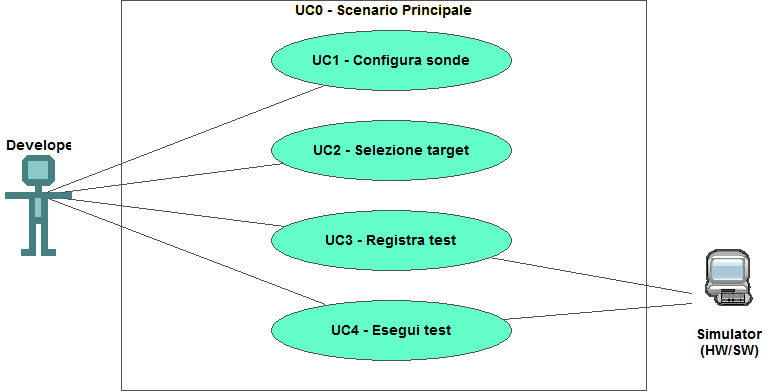
\includegraphics[width=0.9\columnwidth]{usecase/scenario-principale} 
    \caption{Use Case - UC0: Scenario principale}
\end{figure}

\begin{usecase}{0}{Scenario principale}
\usecaseactors{Sviluppatore applicativi}
\usecasepre{Lo sviluppatore è entrato nel plug-in di simulazione all'interno dell'IDE}
\usecasedesc{La finestra di simulazione mette a disposizione i comandi per configurare, registrare o eseguire un test}
\usecasepost{Il sistema è pronto per permettere una nuova interazione}
\label{uc:scenario-principale}
\end{usecase}

\section{Tracciamento dei requisiti}

Da un'attenta analisi dei requisiti e degli use case effettuata sul progetto è stata stilata la tabella che traccia i requisiti in rapporto agli use case.\\
Sono stati individuati diversi tipi di requisiti e si è quindi fatto utilizzo di un codice identificativo per distinguerli.\\
Il codice dei requisiti è così strutturato R(F/Q/V)(N/D/O) dove:
\begin{enumerate}
	\item[R =] requisito
    \item[F =] funzionale
    \item[Q =] qualitativo
    \item[V =] di vincolo
    \item[N =] obbligatorio (necessario)
    \item[D =] desiderabile
    \item[Z =] opzionale
\end{enumerate}
Nelle tabelle \ref{tab:requisiti-funzionali}, \ref{tab:requisiti-qualitativi} e \ref{tab:requisiti-vincolo} sono riassunti i requisiti e il loro tracciamento con gli use case delineati in fase di analisi.

\newpage

\begin{table}[hbt!]
\caption{Tabella del tracciamento dei requisti funzionali}
\label{tab:requisiti-funzionali}
\begin{tabularx}{\textwidth}{lXl}
\hline\hline
\textbf{Requisito} & \textbf{Descrizione} & \textbf{Use Case}\\
\hline
RFN-1     & L'interfaccia permette di configurare il tipo di sonde del test & UC1 \\
\hline
\end{tabularx}
\end{table}%

\begin{table}[hbt!]
\caption{Tabella del tracciamento dei requisiti qualitativi}
\label{tab:requisiti-qualitativi}
\begin{tabularx}{\textwidth}{lXl}
\hline\hline
\textbf{Requisito} & \textbf{Descrizione} & \textbf{Use Case}\\
\hline
RQD-1    & Le prestazioni del simulatore hardware deve garantire la giusta esecuzione dei test e non la generazione di falsi negativi & - \\
\hline
\end{tabularx}
\end{table}%

\begin{table}[hbt!]
\caption{Tabella del tracciamento dei requisiti di vincolo}
\label{tab:requisiti-vincolo}
\begin{tabularx}{\textwidth}{lXl}
\hline\hline
\textbf{Requisito} & \textbf{Descrizione} & \textbf{Use Case}\\
\hline
RVO-1    & La libreria per l'esecuzione dei test automatici deve essere riutilizzabile & - \\
\hline
\end{tabularx}
\end{table}%